% Two landscape A4 pages: (1) inference pipeline, (2) GBLA training workflow.
% Same content as Figures 8 and 9 of complete_research_progress_report.pdf.
% Compile with:  tectonic pipeline_diagrams_landscape.tex
\documentclass[11pt]{article}
\usepackage[a4paper,landscape,margin=14mm]{geometry}
\usepackage{lmodern}
\usepackage{amsmath,amssymb}
\usepackage{xcolor}
\usepackage{tikz}
\usetikzlibrary{arrows.meta,positioning,fit,backgrounds}
\pagestyle{empty}
\setlength{\parindent}{0pt}

\definecolor{box}{HTML}{EEF2F7}
\definecolor{trn}{HTML}{FCE9C8}
\definecolor{frz}{HTML}{DCE6F2}

\tikzset{
  blk/.style={draw,rounded corners=3pt,fill=box,align=center,font=\normalsize,minimum height=19mm,text width=46mm,line width=0.8pt},
  frz/.style={blk,fill=frz},
  trn/.style={blk,fill=trn},
  lab/.style={font=\footnotesize,text=black!80,inner sep=1.5pt},
  ar/.style={-{Latex[length=3mm]},line width=1.1pt}}

\begin{document}

% ---------------------------------------------------------------------
% PAGE 1: inference pipeline
% ---------------------------------------------------------------------
\begin{center}
{\Large\bfseries GBLA / LN-tuned CLIP ViT-L/14 --- Implemented Inference Pipeline}\\[2pt]
{\small Tensor shapes on the arrows. Orange = trained parameters (104,450 = deployed \(\theta_s\)); blue = frozen.}
\end{center}
\vspace{4mm}

\begin{center}
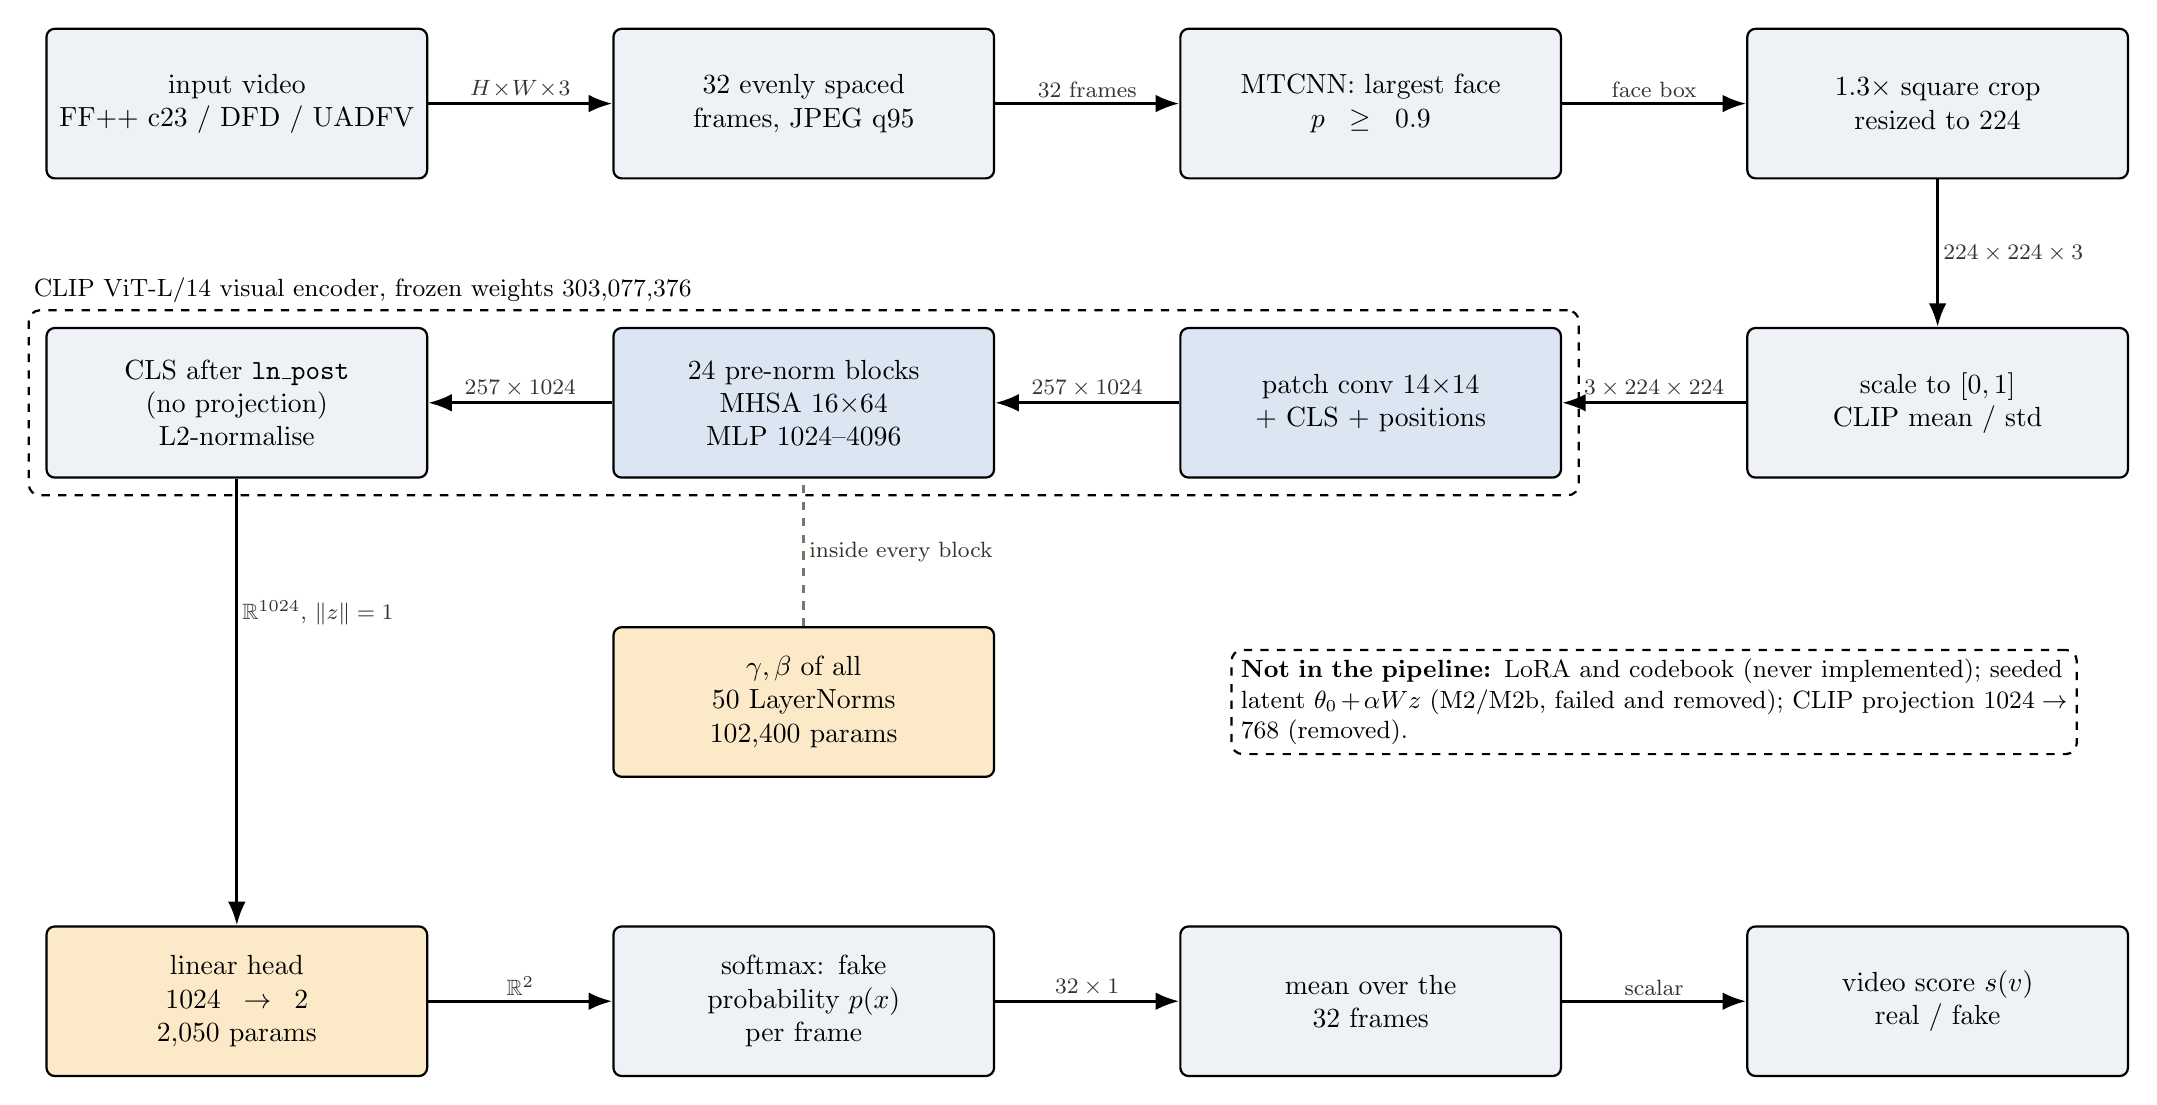
\begin{tikzpicture}[x=72mm,y=-38mm]
% row 1: left to right
\node[blk] (vid) at (0,0) {input video\\FF++ c23 / DFD / UADFV};
\node[blk] (frm) at (1,0) {32 evenly spaced\\frames, JPEG q95};
\node[blk] (det) at (2,0) {MTCNN: largest face\\\(p\ge0.9\)};
\node[blk] (crp) at (3,0) {1.3\(\times\) square crop\\resized to 224};
% row 2: right to left
\node[blk] (pre) at (3,1) {scale to \([0,1]\)\\CLIP mean / std};
\node[frz] (pe)  at (2,1) {patch conv 14\(\times\)14\\+ CLS + positions};
\node[frz] (tr)  at (1,1) {24 pre-norm blocks\\MHSA 16\(\times\)64\\MLP 1024--4096};
\node[blk] (cls) at (0,1) {CLS after \texttt{ln\_post}\\(no projection)\\L2-normalise};
% row 3
\node[trn] (ln)  at (1,2) {\(\gamma,\beta\) of all\\50 LayerNorms\\102,400 params};
\node[draw,dashed,rounded corners,font=\small,align=left,text width=105mm,line width=0.8pt] at (2.5,2)
 {\textbf{Not in the pipeline:} LoRA and codebook (never implemented); seeded latent \(\theta_0+\alpha Wz\) (M2/M2b, failed and removed); CLIP projection \(1024\to768\) (removed).};
% row 4: left to right
\node[trn] (head) at (0,3) {linear head\\\(1024\to2\)\\2,050 params};
\node[blk] (sm)   at (1,3) {softmax: fake\\probability \(p(x)\)\\per frame};
\node[blk] (agg)  at (2,3) {mean over the\\32 frames};
\node[blk] (out)  at (3,3) {video score \(s(v)\)\\real / fake};
% arrows and shapes
\draw[ar] (vid)--node[lab,above]{\(H\!\times\!W\!\times\!3\)}(frm);
\draw[ar] (frm)--node[lab,above]{32 frames}(det);
\draw[ar] (det)--node[lab,above]{face box}(crp);
\draw[ar] (crp)--node[lab,right]{\(224\times224\times3\)}(pre);
\draw[ar] (pre)--node[lab,above]{\(3\times224\times224\)}(pe);
\draw[ar] (pe)--node[lab,above]{\(257\times1024\)}(tr);
\draw[ar] (tr)--node[lab,above]{\(257\times1024\)}(cls);
\draw[ar] (cls)--node[lab,right,pos=0.3]{\(\mathbb{R}^{1024}\), \(\|z\|=1\)}(head);
\draw[ar] (head)--node[lab,above]{\(\mathbb{R}^{2}\)}(sm);
\draw[ar] (sm)--node[lab,above]{\(32\times1\)}(agg);
\draw[ar] (agg)--node[lab,above]{scalar}(out);
\draw[line width=1.1pt,dashed,trn!50!black] (ln)--node[lab,right]{inside every block}(tr);
\begin{scope}[on background layer]
\node[draw,dashed,rounded corners,fit=(pe)(tr)(cls),inner sep=6pt,line width=0.8pt] (bb) {};
\end{scope}
\node[font=\small,anchor=south west,inner sep=2pt] at (bb.north west) {CLIP ViT-L/14 visual encoder, frozen weights 303,077,376};
\end{tikzpicture}
\end{center}

\vfill
{\small During training, augmentation (flip, affine, blur, colour jitter, JPEG 40--100) is applied between cropping and normalisation. Video score \(s(v)=\frac{1}{32}\sum_{t=1}^{32}p(x_t)\).}

\newpage
% ---------------------------------------------------------------------
% PAGE 2: training workflow
% ---------------------------------------------------------------------
\begin{center}
{\Large\bfseries GBLA Training Workflow (M4 onward)}\\[2pt]
{\small Shared \(\theta_s\) plus private offsets \(\delta_g\) per generator; only \(\theta_s\) (104,450 numbers) is deployed.}
\end{center}
\vspace{8mm}

\begin{center}
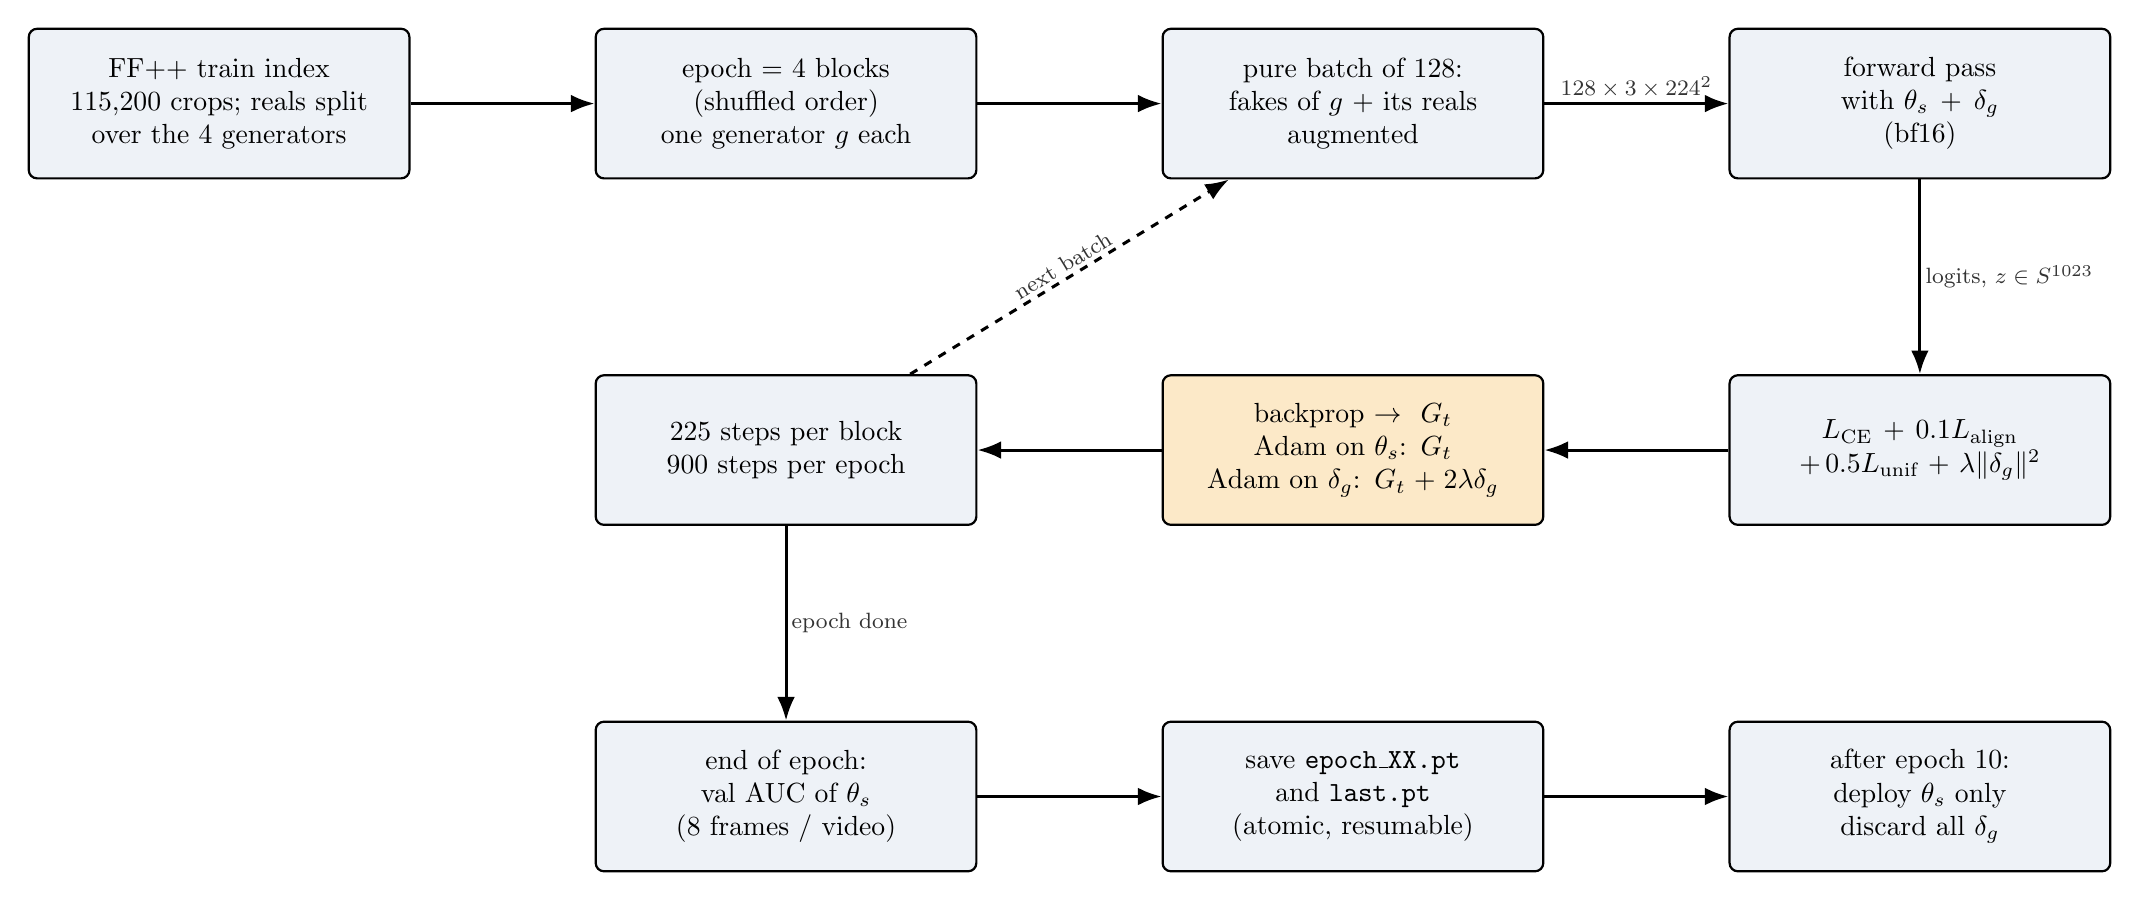
\begin{tikzpicture}[x=72mm,y=-44mm]
\node[blk] (ds)   at (0,0) {FF++ train index\\115,200 crops; reals split\\over the 4 generators};
\node[blk] (blk)  at (1,0) {epoch = 4 blocks\\(shuffled order)\\one generator \(g\) each};
\node[blk] (bat)  at (2,0) {pure batch of 128:\\fakes of \(g\) + its reals\\augmented};
\node[blk] (fw)   at (3,0) {forward pass\\with \(\theta_s+\delta_g\)\\(bf16)};
\node[blk] (loss) at (3,1) {\(L_\text{CE}+0.1L_\text{align}\)\\\(+\,0.5L_\text{unif}+\lambda\|\delta_g\|^2\)};
\node[trn] (bp)   at (2,1) {backprop \(\to G_t\)\\Adam on \(\theta_s\): \(G_t\)\\Adam on \(\delta_g\): \(G_t+2\lambda\delta_g\)};
\node[blk] (nxt)  at (1,1) {225 steps per block\\900 steps per epoch};
\node[blk] (val)  at (1,2) {end of epoch:\\val AUC of \(\theta_s\)\\(8 frames / video)};
\node[blk] (ck)   at (2,2) {save \texttt{epoch\_XX.pt}\\and \texttt{last.pt}\\(atomic, resumable)};
\node[blk] (fin)  at (3,2) {after epoch 10:\\deploy \(\theta_s\) only\\discard all \(\delta_g\)};
\draw[ar] (ds)--(blk); \draw[ar] (blk)--(bat);
\draw[ar] (bat)--node[lab,above]{\(128\times3\times224^2\)}(fw);
\draw[ar] (fw)--node[lab,right]{logits, \(z\in S^{1023}\)}(loss);
\draw[ar] (loss)--(bp); \draw[ar] (bp)--(nxt);
\draw[ar,dashed] (nxt)--node[lab,above,sloped]{next batch}(bat);
\draw[ar] (nxt)--node[lab,right]{epoch done}(val);
\draw[ar] (val)--(ck); \draw[ar] (ck)--(fin);
\end{tikzpicture}
\end{center}

\vfill
{\small With \(\lambda=\infty\) the offsets stay zero, which is pooled training with pure-generator batches; M1 (the LNCLIP-DF baseline) used mixed batches and no offsets. Chosen \(\lambda=0.01\). Optimiser AdamW (no weight decay), learning rate 1 warm-up epoch \(10^{-5}\to3\times10^{-4}\), cosine back to \(10^{-5}\). No checkpoint is selected by validation or test performance.}

\end{document}
